\documentclass[main]{subfiles}
\begin{document}

\section*{Lecture 13 // Oct 6 // Defining Instanton Floer Homology}
\addcontentsline{toc}{section}{Lecture 13 -- Defining Instanton Floer Homology}

Last time: we restricted to $Y^3$ a $\mathbb{Z}\mathrm{HS}^3$, and fixed the (trivial) $\SU(2)$ bundle $E$ over $Y$. Let $\mc{A}^{\mathrm{irr}}\subset \mc{A}$ be the subset of connections with stabilizer $\pm I$.

Define
\[
\mc{B} = \underbrace{\mc{A}}_{\SU(2) \text{ connections}} / \underbrace{\mc{G}}_{\text{gauge group}}, \qquad \mc{B}^\ast = \mc{A}^{\mathrm{irr}}/\mc{G}.
\]

Then the Chern-Simons Functional is a map $\CS : \mc{B}\to \mathbb{R}/\mathbb{Z}$.

\begin{definition}[IFH, irreducible complex]
\[
C(Y) = \mathbb{F}\langle \text{crit points of CS on } \mc{B}^\ast\rangle.
\]
\end{definition}

\begin{remark}
We have to perturb CS to ensure that the critical points are isolated. This perturbation happens in the same way one perturbs a function $f: M\to \mathbb{R}$ to be Morse.
\end{remark}

Since $\mc{G}$ has $\mathbb{Z}$-many path components, $\pi_0(\mc{G}_0)=\mathbb{Z}$, so $\pi_1(\mc{B}^\ast)=\mathbb{Z}$. Now, take $x,y\in\Crit(\CS)$ and let $\gamma$ be a path from $x$ to $y$ in $\mc{B}$.

The set of homotopy classes of such paths is $\mathbb{Z}$.

\begin{definition}
The moduli space of $\gamma$-flow lines from $x$ to $y$ is
\[
\mc{M}_\gamma(x,y) = \left\{
\begin{array}{l}
\text{ASD connections on } Y\times I \\
\text{which limit to } x \text{ and } y \text{ on each} \\
\text{end and lie in homotopy class of } \gamma
\end{array}
\right\} \Big/ \text{ gauge transformations on } Y\times I.
\]
\end{definition}

\begin{center}
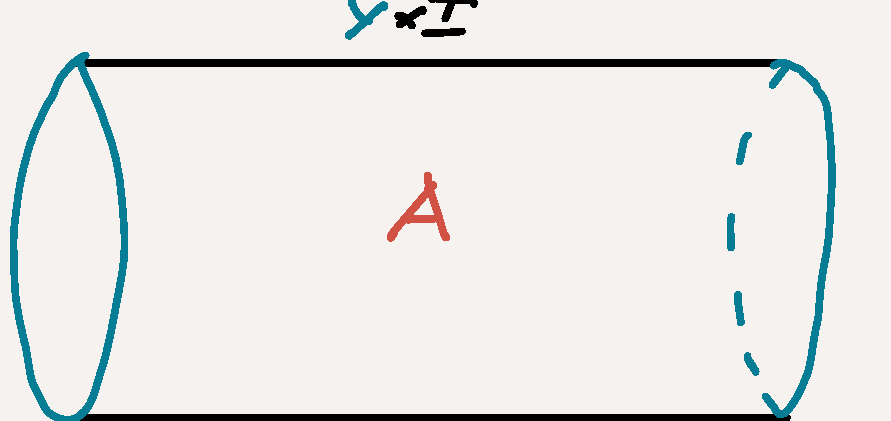
\includegraphics[width=0.55\linewidth]{figures/fig_lec13_cylinder_A.png}
\end{center}

Note that there is a free $\mathbb{R}$ action on $\mc{M}_\gamma(x,y)$ by translation. If you've seen Morse theory, you know where this is going: we'll first quotient by $\mathbb{R}$, then count flowlines.

\begin{definition}
$\mathring{\mc{M}}_\gamma(x,y) = \mc{M}_\gamma(x,y)/\mathbb{R}$,
\[
\partial x = \sum_y \sum_{\gamma\in S} \left|\mathring{\mc{M}}_\gamma(x,y)\right| y,
\]
where $S$ is the set of homotopy classes of paths from $x$ to $y$ for which $\dim(\mathring{\mc{M}}_\gamma(x,y)) = 0$.
\end{definition}

It turns out that, in contrast to finite-dimensional Morse theory, the $\dim(\mathring{\mc{M}}_\gamma(x,y))$ depends on $\gamma$: different homotopy classes of path $\gamma$ from $x$ to $y$ give different dimensional moduli spaces. In particular, the expected dimensions of the ASD moduli spaces differ by $8$. Thus $C(Y)$ is a relatively $\mathbb{Z}/8$-graded complex. The relative grading difference between $x$ and $y$ is
\[
\mathrm{gr}(x)-\mathrm{gr}(y) = \dim(\mc{M}(x,y)) \mod 8.
\]

To get an absolute $\mathbb{Z}/8$ grading on $\CS(Y)$, recall that for $Y$ a $\mathbb{Z}\mathrm{HS}^3$, there is a unique (up to gauge) reducible flat connection on $Y$. Denote this connection by $\Theta$, and define absolute gradings by counting flows into $\Theta$.

\begin{definition}
The absolute grading of $x\in \Crit(\CS)$ is
\[
\mathrm{gr}(x) := \dim(\mc{M}(x,\Theta)) \mod 8.
\]
\end{definition}

However, something goes wrong when we try to include $\Theta$ as a generator of our chain complex. To see this, let's add $\Theta$. Since the boundary map $\partial$ is only defined for irreducible critical points, we must define new boundary maps for flows into and out of $\Theta$. These are Donaldson's $D_1$ and $D_2$ maps.

\begin{definition}
$D_1 : C(Y)\to \mathbb{F}$ (think of as $\mathbb{F}\langle \Theta\rangle$),
\[
D_1(x) = \sum_{\substack{\gamma \text{ from } x \text{ to } \Theta \\ \text{s.t. } \dim(\mc{M}(x,\Theta))=1}} \left|\mc{M}(x,\Theta)/\mathbb{R}\right|.
\]
\end{definition}

\begin{definition}
$D_2 : \mathbb{F}\to C(Y)$,
\[
D_2(1) = \sum_y \left(\sum_{\substack{\gamma \text{ from } \Theta \text{ to } y \\ \text{s.t. } \dim(\mc{M}(\Theta,y))=1}} \left|\mc{M}(\Theta,y)/\mathbb{R}\right|\, y\right).
\]
\end{definition}

Notice that $D_1$ is supported on $C_1(Y) = \{x\in C(Y) \text{ s.t. } \mathrm{gr}(x)=1\}\subset C(Y)$, since the only points which could flow into $\Theta$ must have grading $1$. However, it turns out that $D_2$ has image in $C_{(4)}(Y)$. This is strange.

Let's go back to our definition of relative gradings. Why were these well-defined? The implicit claim here was that for $x,y,z\in\Crit(\CS)$,
\[
\dim(\mc{M}(x,y)) + \dim(\mc{M}(y,z)) = \dim(\mc{M}(x,z)).
\]
E.g., we can construct a flow from $x$ to $z$ by gluing flows from $x\to y$ to flows from $y\to z$.

\begin{center}
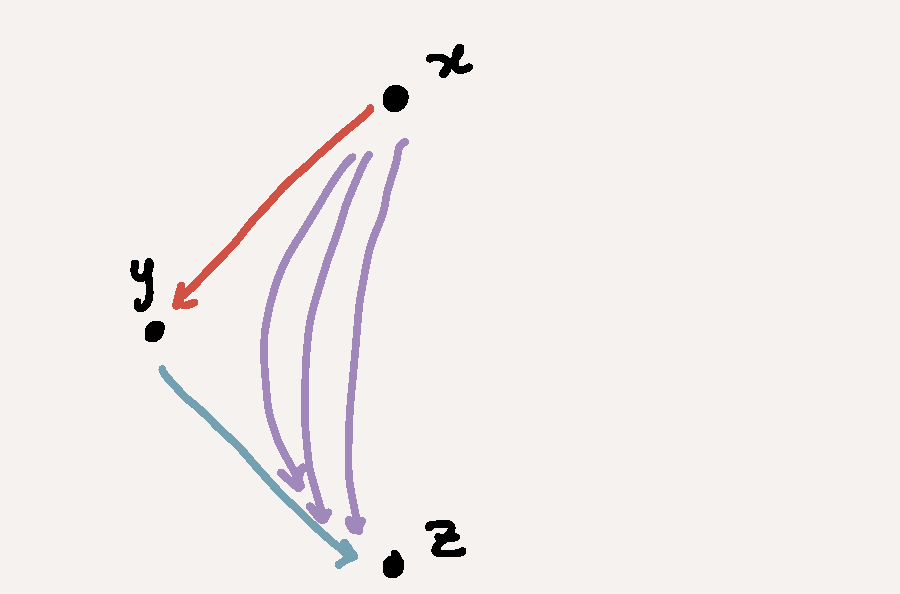
\includegraphics[width=0.22\linewidth]{figures/fig_lec13_tree_xyz.png}
\end{center}

But something goes wrong in the Instanton Floer complex when $y=\Theta$. Say we believe in some gluing procedure. Then, given an ASD connection $A_1$ on $Y\times\mathbb{R}$ which limits to $x$ as $t\to -\infty$ and $y$ as $t\to\infty$, and similarly an $A_2$ from $y$ to $z$, we'd want a connection $A_1\ast A_2$ from $x$ to $z$ on $Y\times\mathbb{R}$ built from $A_1$ and $A_2$.

\begin{center}
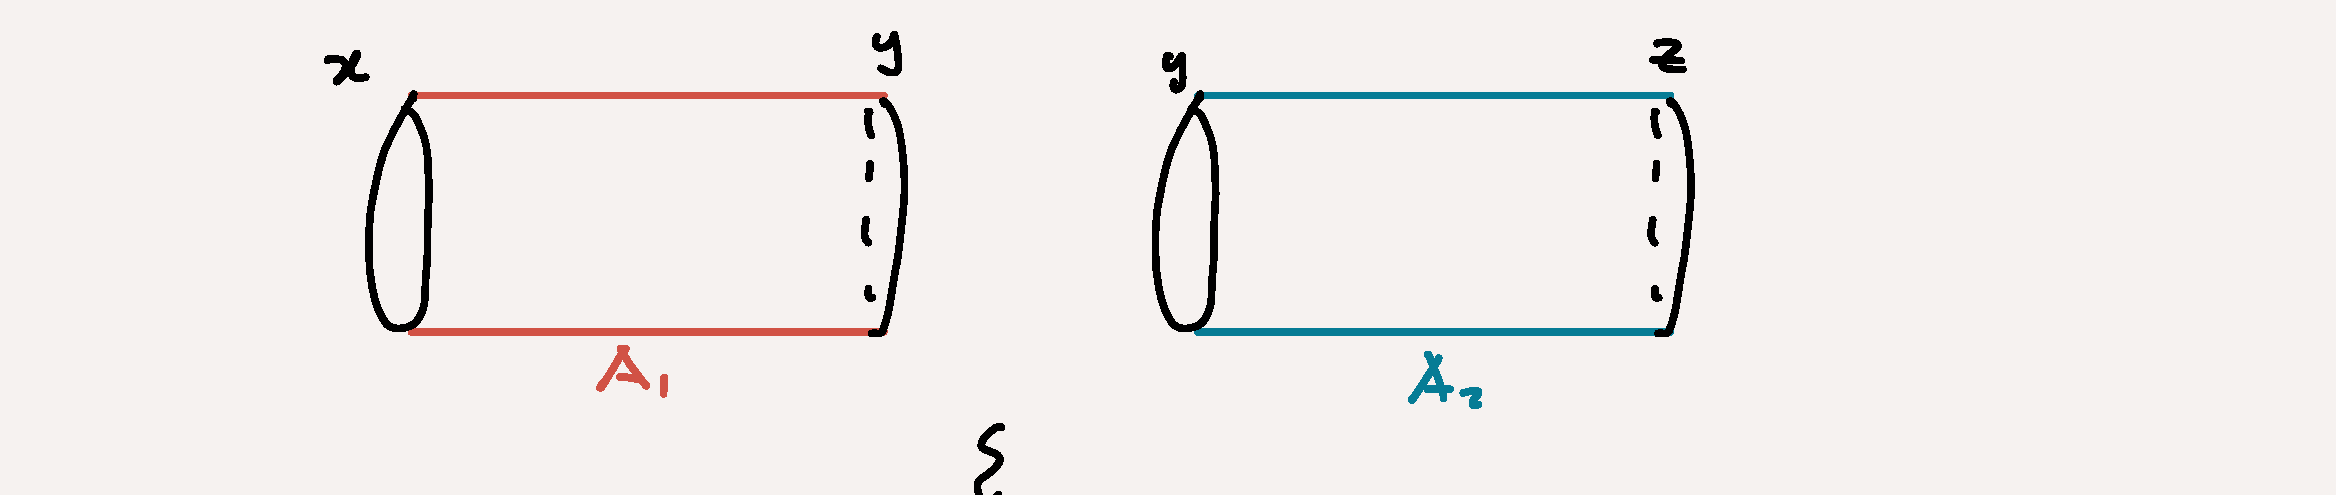
\includegraphics[width=0.9\linewidth]{figures/fig_lec13_cyl_A1_A2.png}
\end{center}

\begin{center}
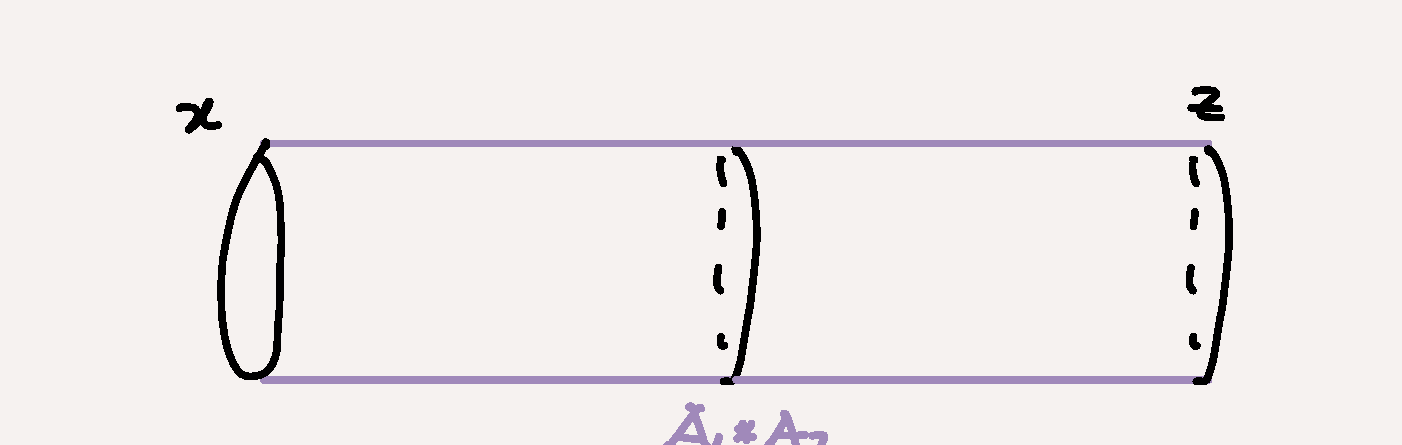
\includegraphics[width=0.6\linewidth]{figures/fig_lec13_cyl_glued.png}
\end{center}

To ``glue'' $A_1$ and $A_2$ together at $y$ to get something smooth, we'll need to add a decay function that ensures that after a certain time $T$,
\[
f\circ A_1|_{[T,\infty)} = f\circ A_2|_{(-\infty,T]}.
\]

\begin{center}
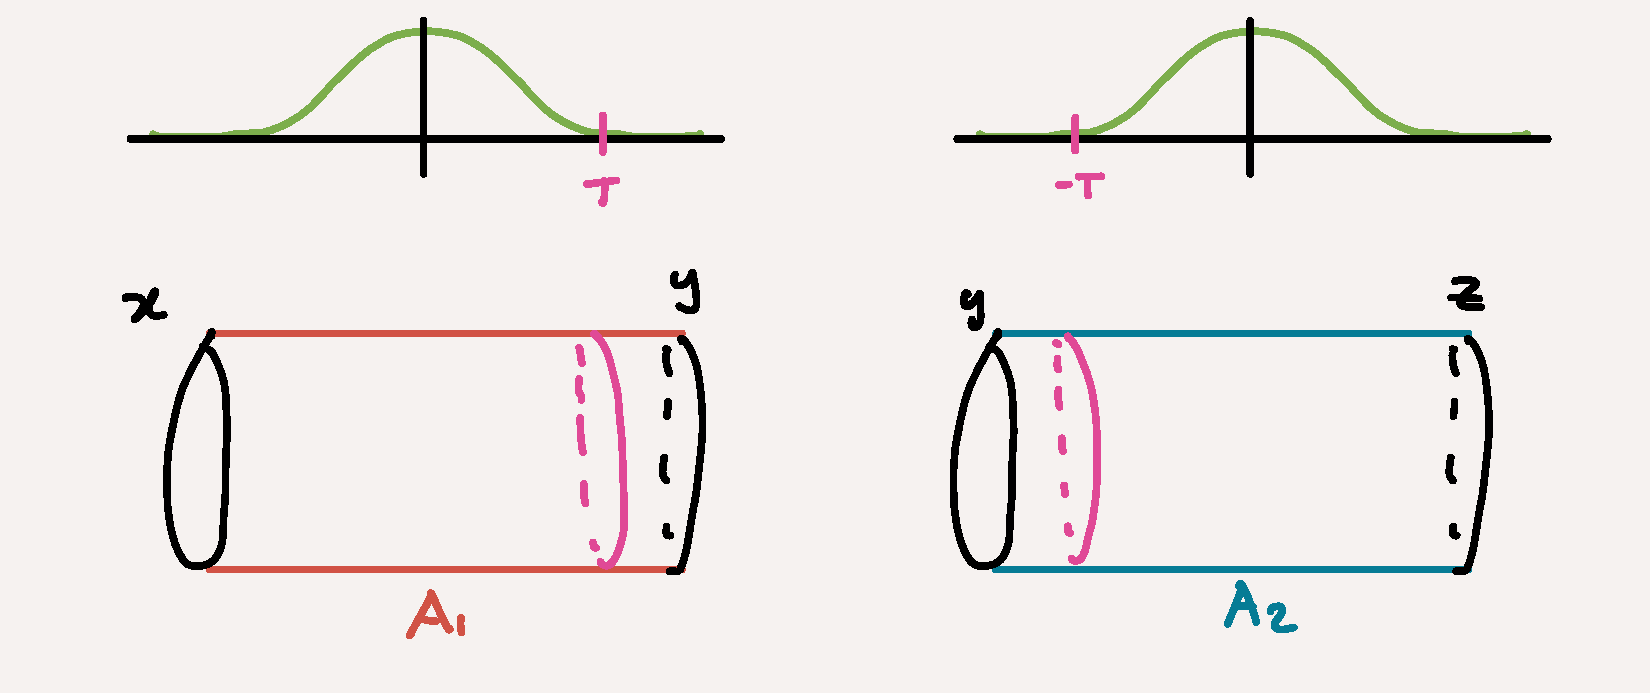
\includegraphics[width=0.9\linewidth]{figures/fig_lec13_bump_individual.png}
\end{center}

\begin{center}
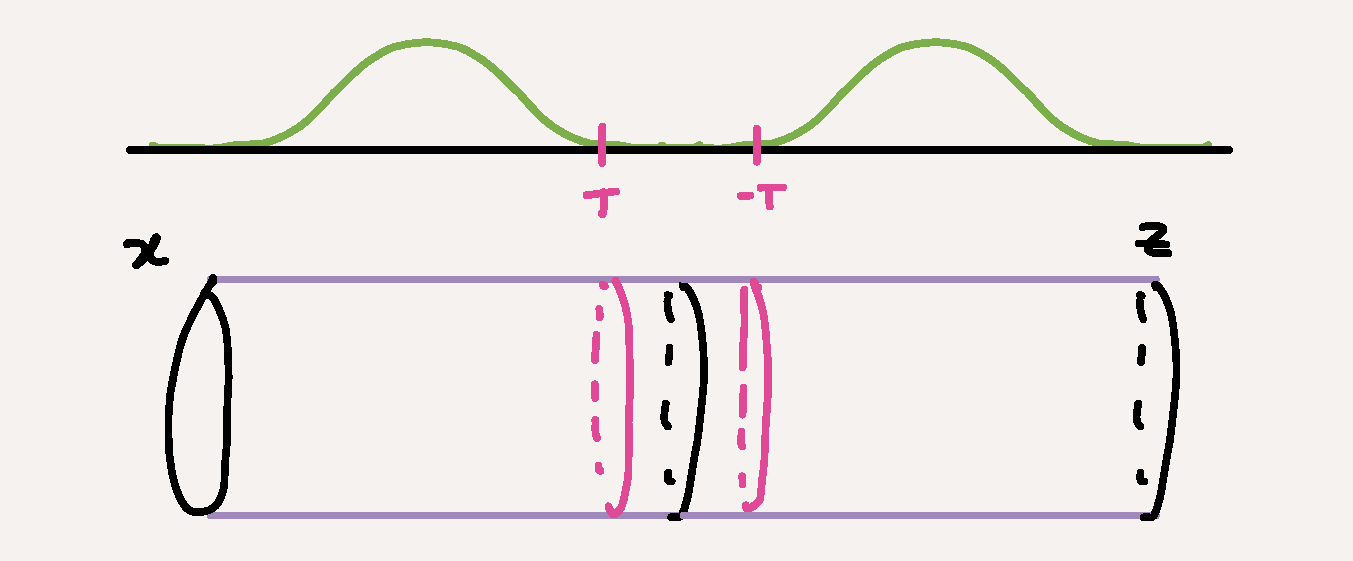
\includegraphics[width=0.55\linewidth]{figures/fig_lec13_bump_combined.png}
\end{center}

This gives us a $1$-dimensional gluing parameter $T$. In the flowline picture, the analog is building a flowline from $x$ to $z$ by choosing a cutoff parameter, following $x\to y$ until then,

\begin{center}
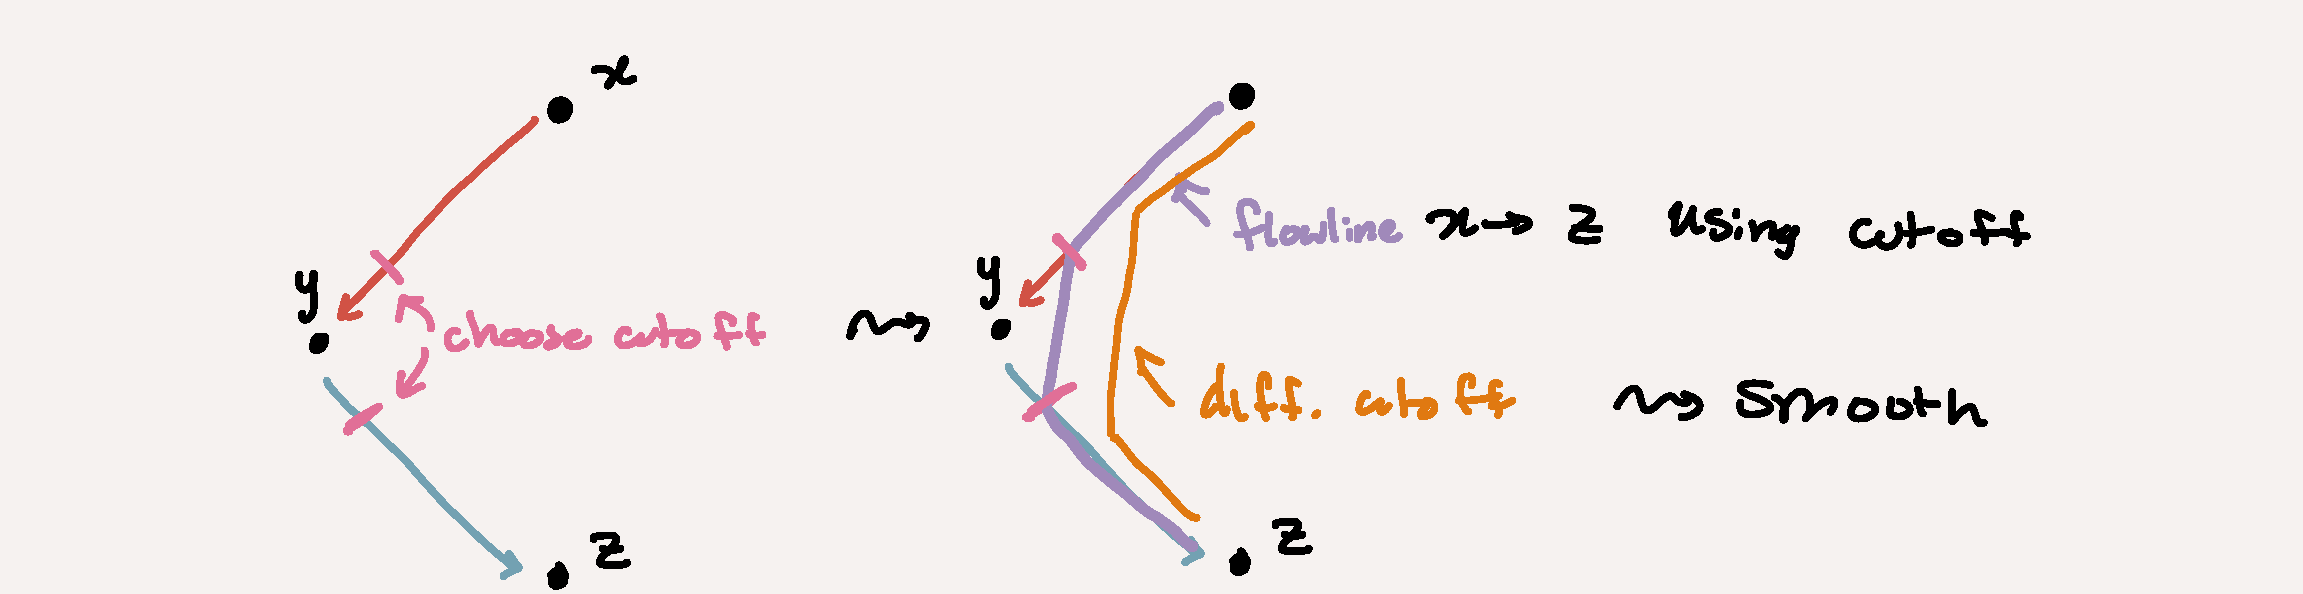
\includegraphics[width=0.9\linewidth]{figures/fig_lec13_cutoff_flowlines.png}
\end{center}

What goes wrong when $y$ has large stabilizer? To glue, we can pick representatives on each end which are literally the same. But we can also compose with gauge transformations to get new gluings.

\begin{center}
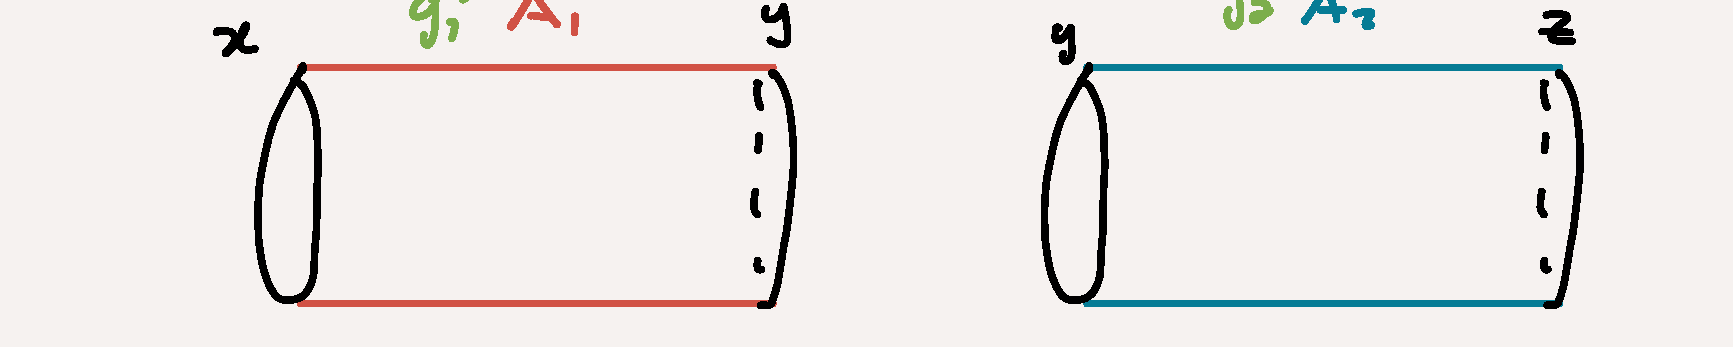
\includegraphics[width=0.75\linewidth]{figures/fig_lec13_cyl_gauge.png}
\end{center}

If $g_1^\ast A_1|_y = g_2^\ast A_2|_y$, then the connection on the composite cylinder is gauge-equivalent to the original connection glued via the identity.

But if $\Stab(y)$ is big, we get many more connections on $Y\times\mathbb{R}$ than we would expect!

$c = $ constant, non-identity gauge transformation on $A_2$.

\begin{center}
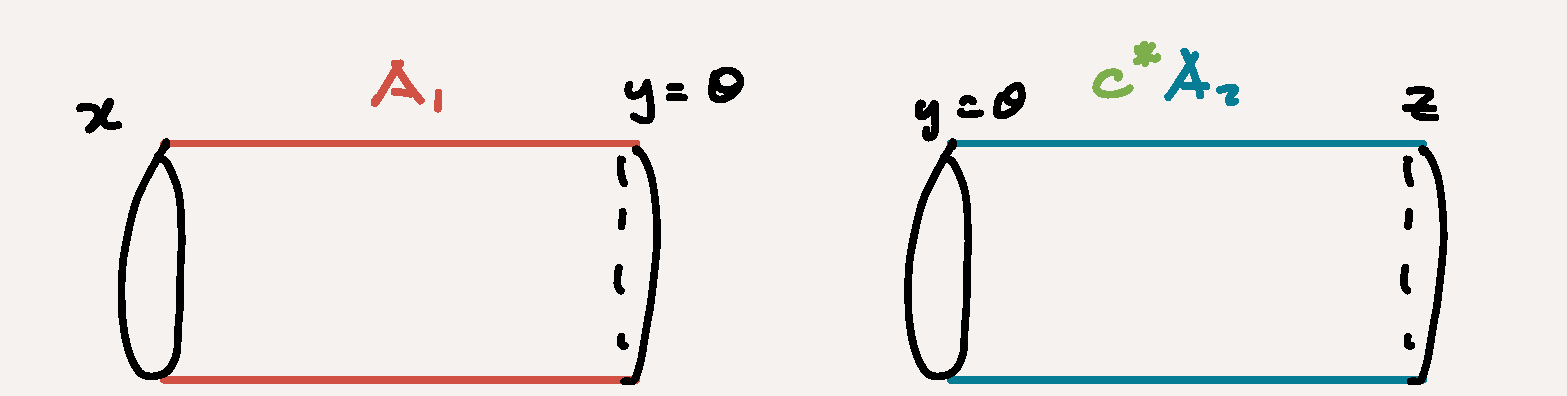
\includegraphics[width=0.6\linewidth]{figures/fig_lec13_cyl_stab.png}
\end{center}

Since $y$ has big stabilizer, $c^\ast(A_2)|_y = A_2|_y$, so we can still glue to get a connection on the entire composite cylinder. However, $A_1\ast c^\ast A_2$ is not gauge equivalent to $A_1\ast A_2$, since any gauge transformation $c^\ast A_2 \to A_2$ must change $A_1$ as well. Therefore, we get a $\Stab(y)$'s worth of extra distinct connections on $A_1\ast A_2$. Since $y=\Theta$, and $\Stab(\Theta)\cong \SU(2)$,
\[
\dim(\mc{M}(x,z)) = \dim(\mc{M}(x,y)) + \dim(\mc{M}(y,z)) + \dim(\SU(2)) = \dim(\mc{M}(x,y)) + \dim(\mc{M}(y,z)) + 3.
\]

This exactly matches what was claimed earlier: for $D_1 : x\to y$, $D_2 : y\to z$, we expect a grading difference of $2$ for $x\to z$, but $1-(-4)=5=2+3$.

Another important fact is that in general, $D_2\circ D_1\neq 0$. This is in contrast with finite-dimensional Morse theory, where $\partial^2(x)=0$ for all $x$. Let's recall why this is true.
\[
\partial^2(x) = \partial(\partial(x)) = \partial\left(\sum_{\substack{y\in C_{k-1}}} n(x,y)\, x\atop{\#\text{flows } x\to y}\right) = \sum_{z\in C_{k-2}}\left(\sum_{y\in C_{k-1}} n(x,y)\, n(y,z)\right) y.
\]

$\partial^2(x)$ breaks up as a sum of terms $cz$, where $c$ is the number of broken flowlines from $x$ to $z$.
\[
\partial^2(x) = \sum \cdots + cz + \cdots,
\]
The claim is that the coefficient $c$ is always $0$. Indeed, the moduli space $\mc{M}(x,z)/\mathbb{R}$ is a $2$-dimensional manifold$/\mathbb{R}$, so it is an open $1$-manifold. It admits a compactification, where the endpoints are broken flowlines. Thus the number of broken flowlines is even. Thus zero mod $2$, and with slightly more work, one can show the signed count is also zero.

However, this relies on the fact that $\mc{M}(x,z)$ is a $2$-dimensional manifold, which comes from the index difference of $2$. Therefore this argument fails for $\Theta$ in IFH, so we can't add in the reducible and get a chain complex. But $D_1\circ\partial = 0$ and $\partial\circ D_2 = 0$, so there's some hope of working around this. One such way is by augmenting.

Note that $D_2(\Theta)$ is a cycle in $C(Y)$, and thus defines a homology class $[D_2(\Theta)]\in H_{-4}(C)$. $D_1$ defines a cohomology element since it vanishes on $\mathrm{im}(\partial)$, so $[D_1]\in H^1(C)$.

Given the irreducible complex $C$ with $D_1$ and $D_2$, we can define the reducible complex by either precomposing $D_2$ or postcomposing $D_1$ with $\partial$, i.e., we only allow either flows into or out of $\Theta$.

\begin{definition}
The ``upper bar complex'' is $\overline{C} = (C\oplus \mathbb{F}_{(0)}, \ \overline{\partial} = \partial + D_1)$.

The ``lower bar complex'' is $\underline{C} = (C\oplus \mathbb{F}_{(-3)}, \ \underline{\partial} = \partial + D_2)$.
\end{definition}

\begin{center}
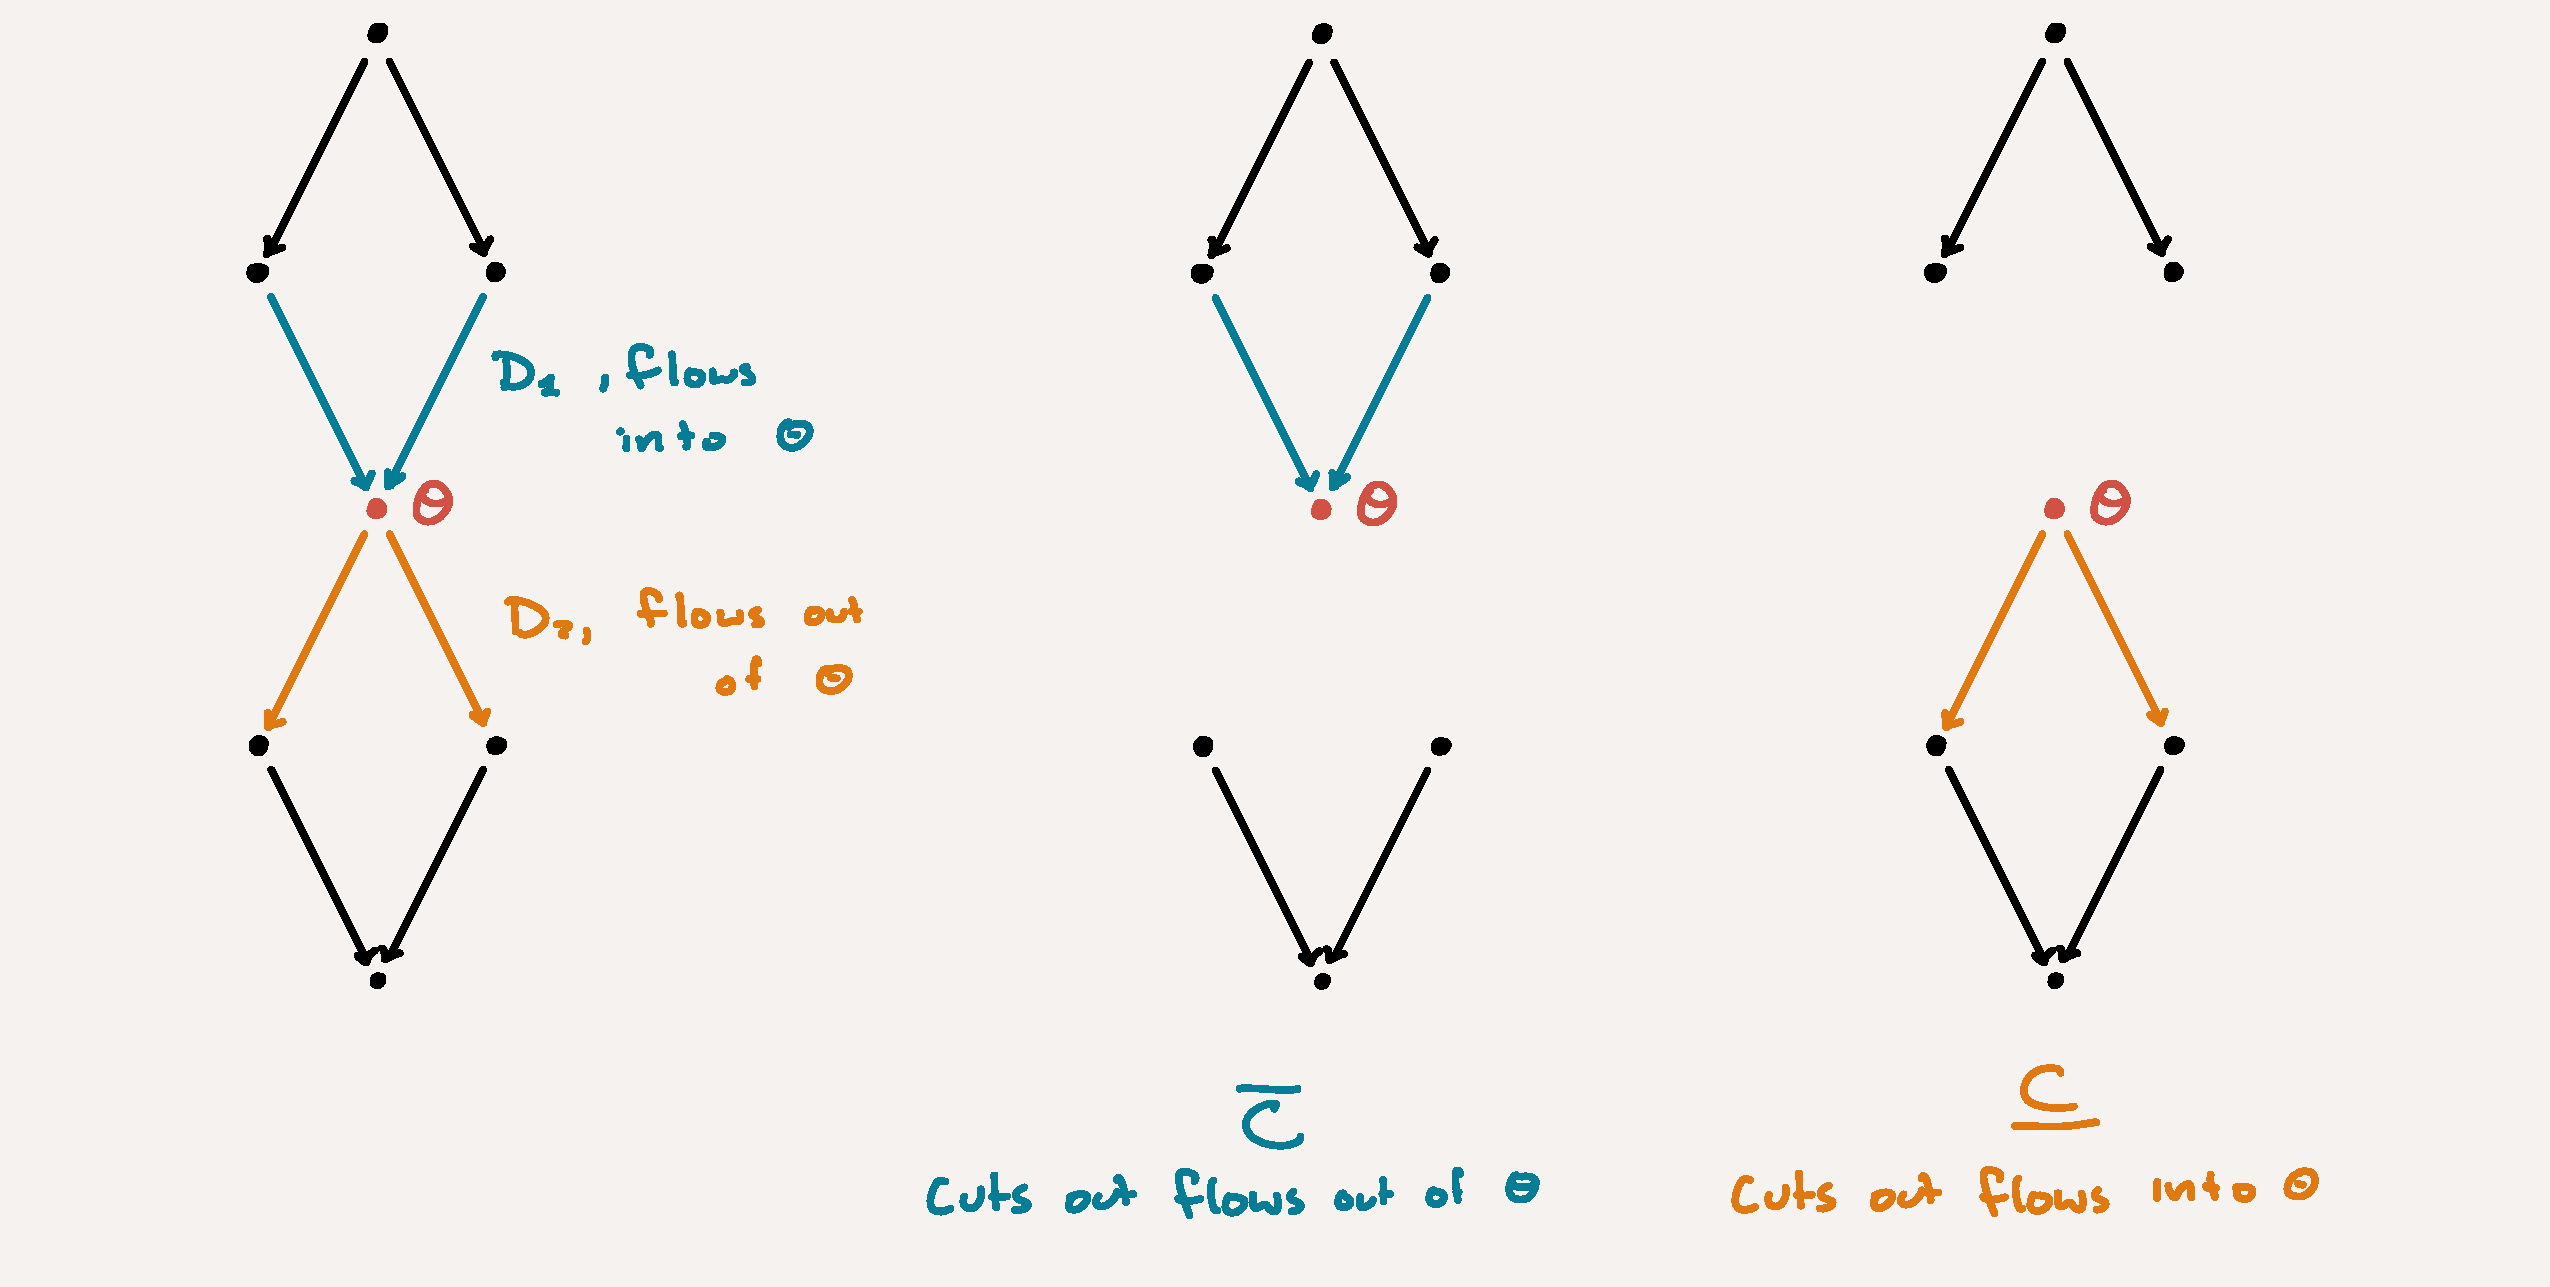
\includegraphics[width=\linewidth]{figures/fig_lec13_bar_complexes.png}
\end{center}

\end{document}
